\documentclass[parskip=half,DIV=12]{scrartcl}

\title{Lab assignment 3}
\subtitle{ATM S 544}
\author{Dominik Stiller}
\date{\today}

\usepackage[english]{babel}
\usepackage[utf8]{inputenc}
\usepackage{siunitx,amsmath,physics}
\usepackage{caption,subcaption,graphicx,csquotes,xcolor}
\usepackage{booktabs}
\usepackage{placeins}
\usepackage[
	backend=biber,
	bibwarn=true,
	bibencoding=utf8,
	sortlocale=en_US,
	url=false,
	style=apa,
	isbn=false
]{biblatex}

\definecolor{uw-purple}{RGB}{51, 0, 111}

\usepackage{hyperref}
\hypersetup{
	% hidelinks,
	colorlinks=true,
	linkcolor=black,
	citecolor=black,
	urlcolor=uw-purple
}

\usepackage{doi}
\usepackage{nomencl}
\makenomenclature
\usepackage[noabbrev,capitalise]{cleveref}
\usepackage[acronym,nonumberlist,nopostdot,nogroupskip]{glossaries}
\usepackage[
	outputdir=build,
]{minted}
\setminted{
	linenos,
	tabsize=4,
	fontsize=\small,
}
\newmintinline{python}{}

\usepackage{lmodern}
\usepackage[T1]{fontenc}
\usepackage{inconsolata}
\usepackage{tikz}

\newcommand{\result}[1]{\colorbox{uw-purple}{\textcolor{white}{#1}}}

\setlength{\nomlabelwidth}{1.5cm}
\setlength{\nomitemsep}{-\parsep}
\newcommand{\nomunit}[1]{%
\renewcommand{\nomentryend}{\hspace*{\fill}\si{#1}}}

\sisetup{per-mode=symbol}
\AtBeginDocument{\RenewCommandCopy\qty\SI}

\DeclareGraphicsRule{.ai}{pdf}{.ai}{}

\addbibresource{bibliography.bib}



\begin{document}

\maketitle




\section{Single observation}

\begin{figure}[h]
    \centering
 
    \begin{subfigure}[c]{\textwidth}
       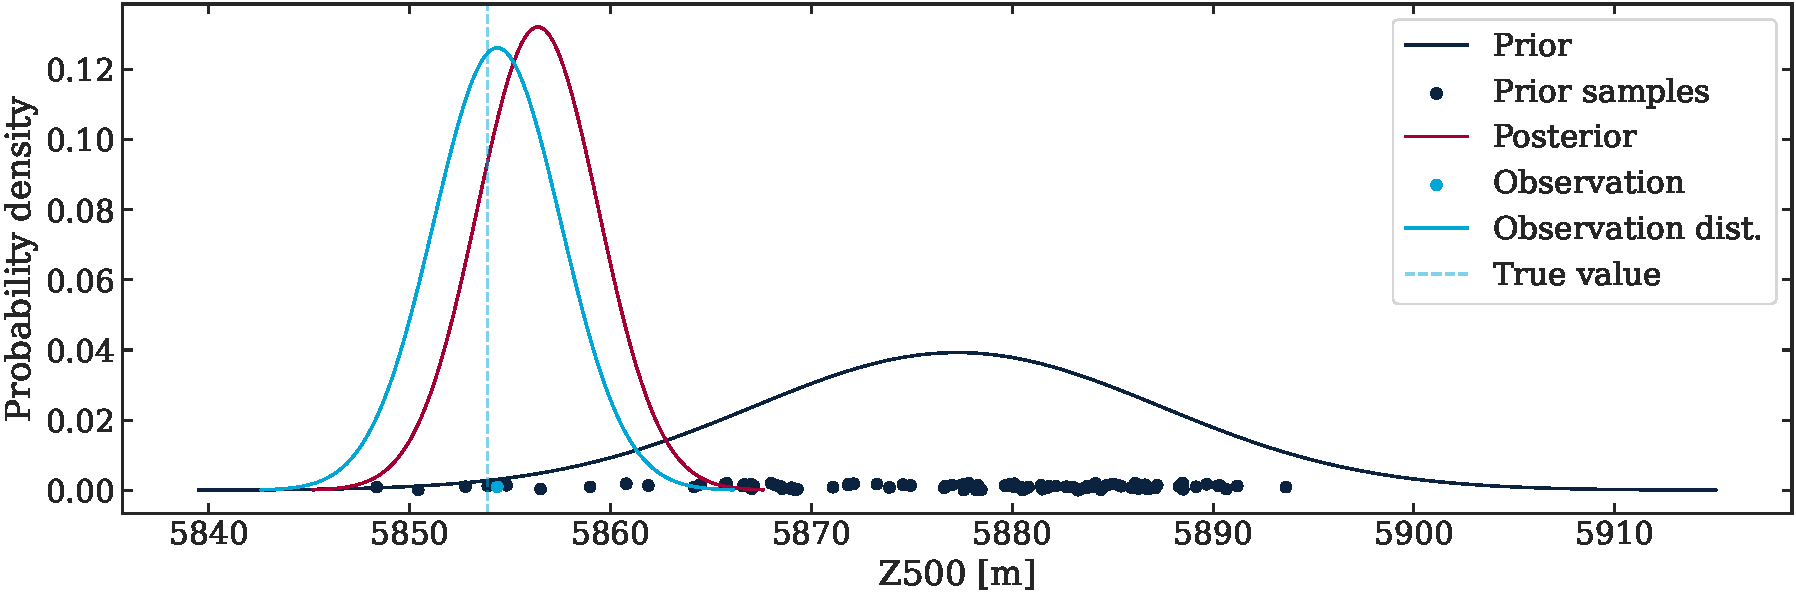
\includegraphics[width=\textwidth]{figures/single_point1.pdf}
       \subcaption{Point 1 (\ang{40} N)}
    \end{subfigure}
     
    \bigskip
     
    \begin{subfigure}[c]{\textwidth}
       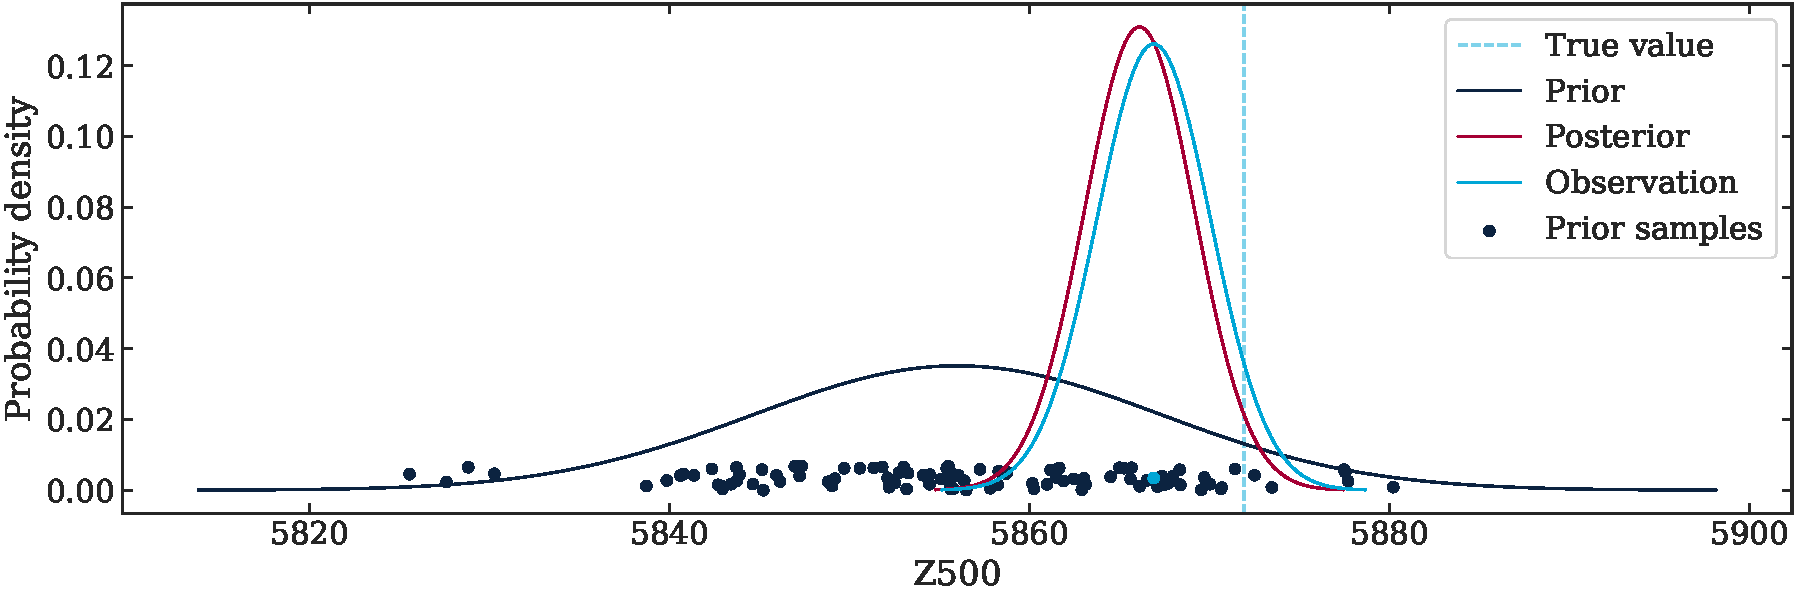
\includegraphics[width=\textwidth]{figures/single_point2.pdf}
       \subcaption{Point 2 (\ang{20} N)}
    \end{subfigure}
 
    \caption{Assimilation of a single observation.}
 \end{figure}



\section{Multiple observations}

\begin{figure}[h]
   \centering

   \begin{subfigure}[c]{\textwidth}
      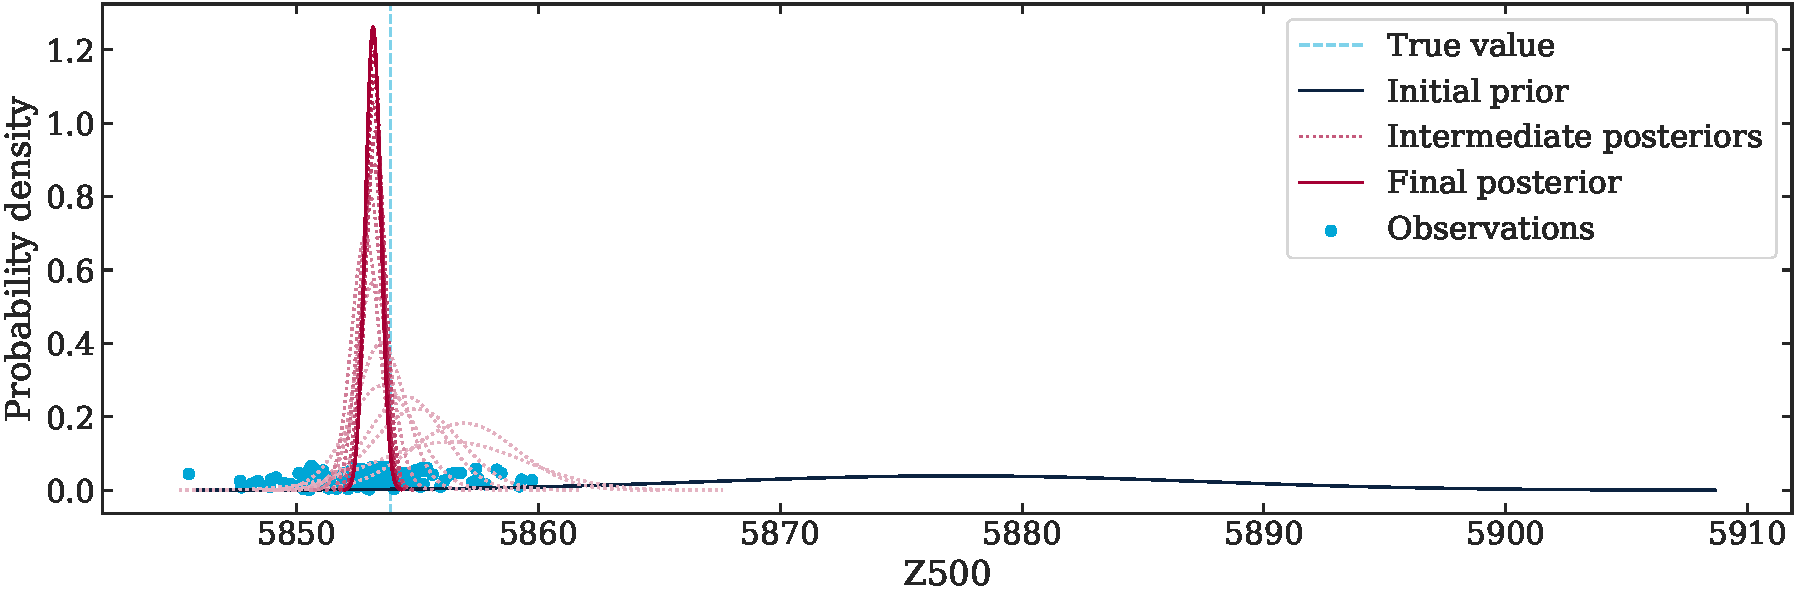
\includegraphics[width=\textwidth]{figures/multiple_point1_var10.pdf}
      \subcaption{Point 1 (\ang{40} N)}
   \end{subfigure}
    
   \bigskip
    
   \begin{subfigure}[c]{\textwidth}
      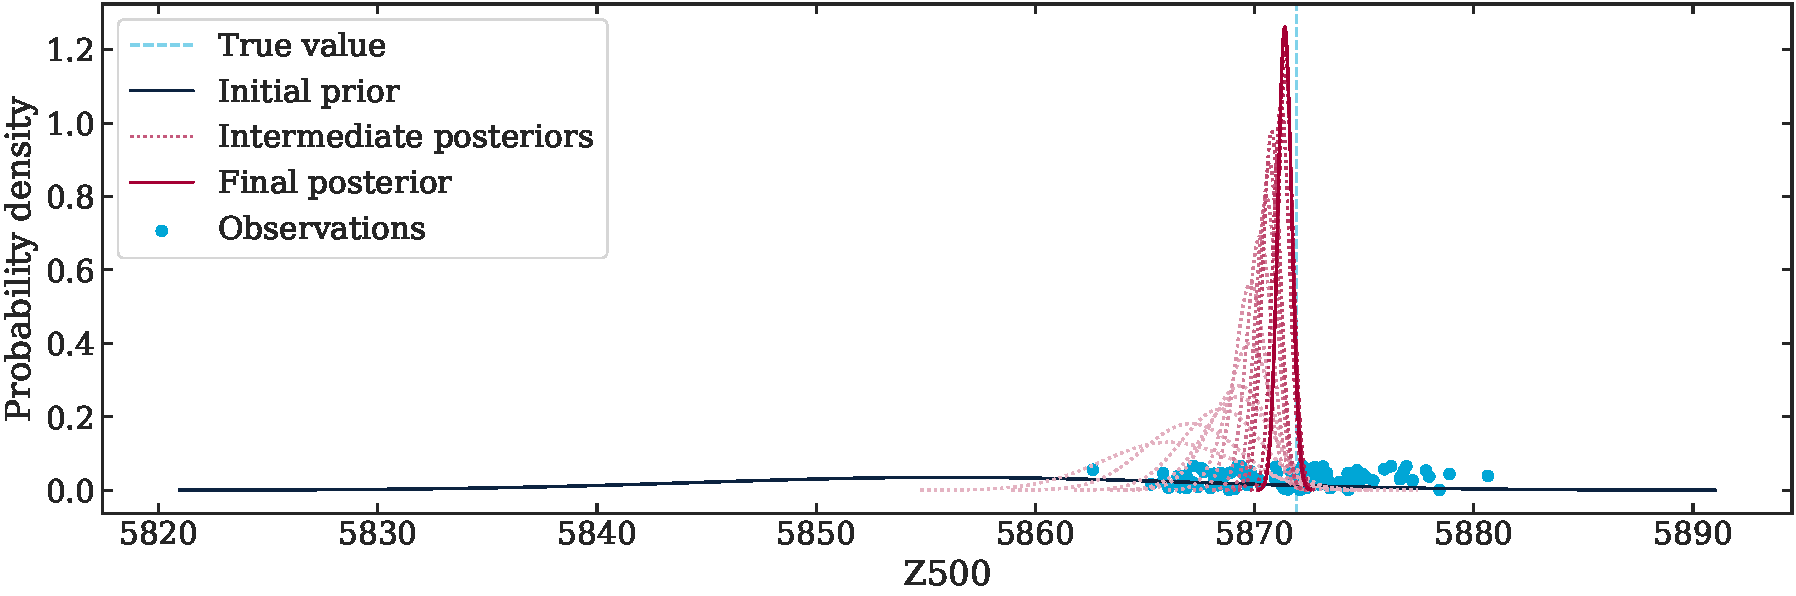
\includegraphics[width=\textwidth]{figures/multiple_point2_var10.pdf}
      \subcaption{Point 2 (\ang{20} N)}
   \end{subfigure}

   \caption{Assimilation of 100 observations.}
\end{figure}


no cos lat weighting because we're only comparing values at the same latitude, and we are only interested in the relative magnitude of error and variance



\subsection{Evolution of error and variance}

\begin{figure}[h]
   \centering

   \begin{subfigure}[c]{\textwidth}
      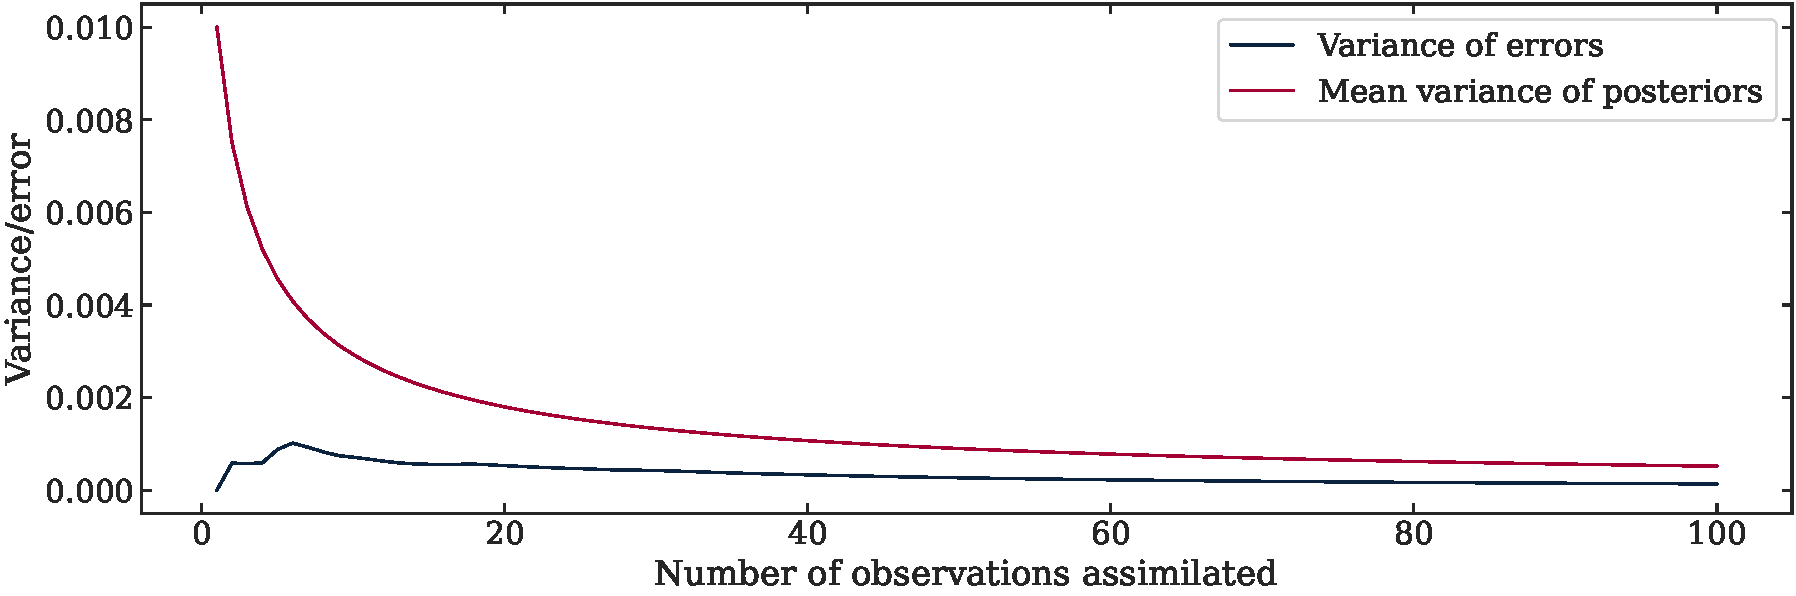
\includegraphics[width=\textwidth]{figures/stats_point1_var01.pdf}
      \subcaption{Point 1 (\ang{40} N)}
   \end{subfigure}
    
   \bigskip
    
   \begin{subfigure}[c]{\textwidth}
      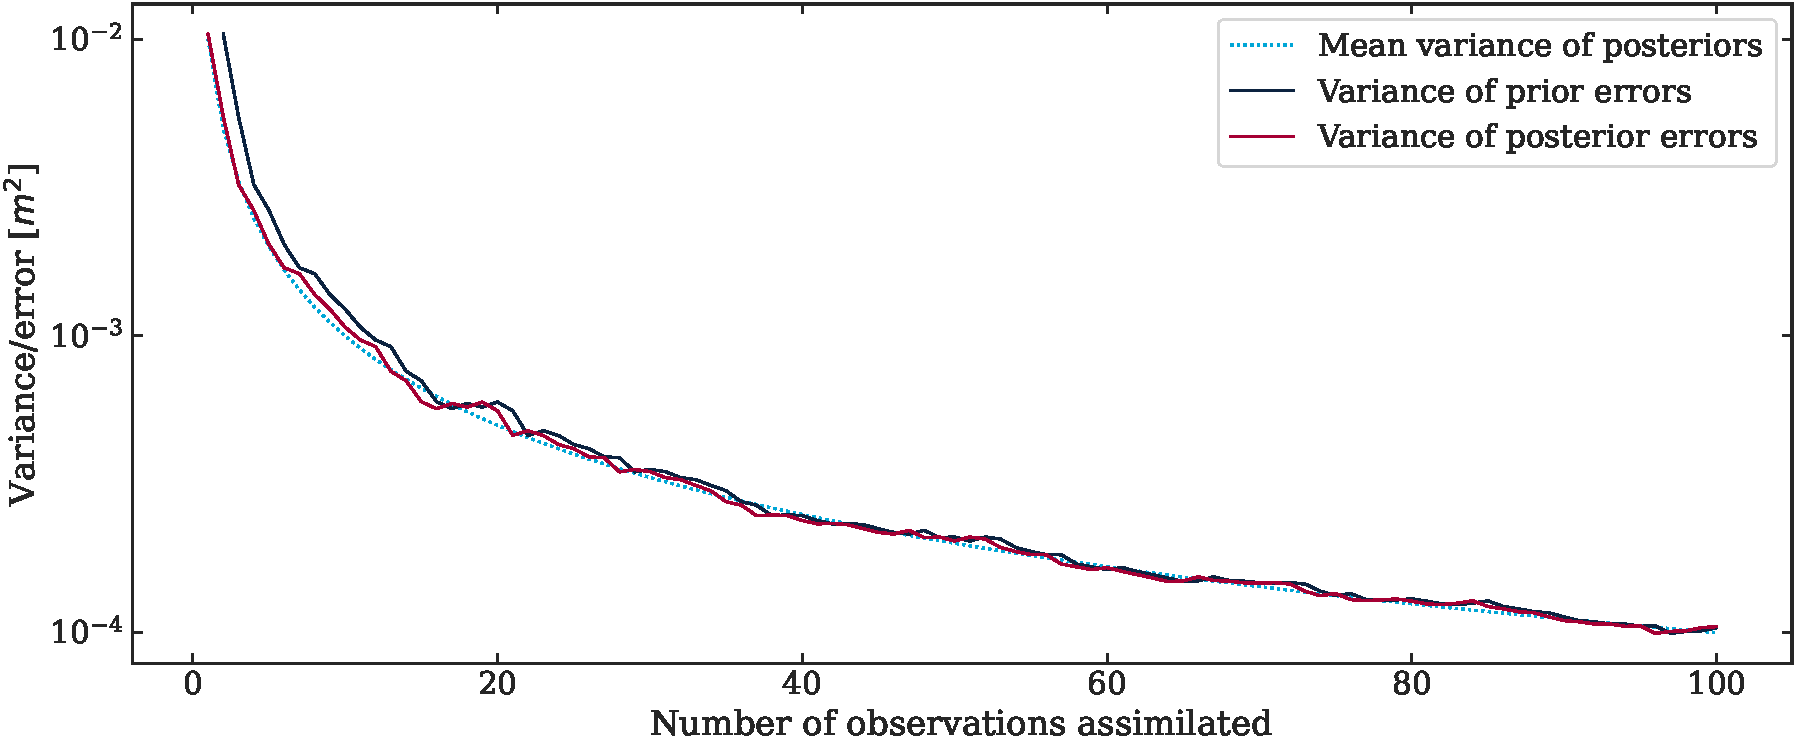
\includegraphics[width=\textwidth]{figures/stats_point2_var01.pdf}
      \subcaption{Point 2 (\ang{20} N)}
   \end{subfigure}

   \caption{Evolution of statistics for assimilation of 100 observations.}
\end{figure}
 



\end{document}
